\documentclass[0-thesis.tex]{subfiles}

\begin{document}
\label{chap:profiles}

\section{DTLS/CoAP profile}
\label{sec:dtls-coap-profile}
% For when discussing ACE:
How clients can access a protected resource through authorization tokens is described in
\parencite{ace} and Figure \ref{fig:ace-flow} shows an adaptation of the protocol flow
from that document. The figure shows a client wanting to access a resource requesting a
token from an authorization server. The token is returned to the client, which can then
send a request with the token to the server holding the resource. If necessary, the
resource server can send an introspection request to the authorization server asking for
more information about the token in order to verify it. If everything goes as planned, the
client is allowed the resource.

\begin{figure}
    \caption{The protocol flow of ACE. Adapted from \parencite{ace}.}
    \label{fig:ace-flow}
    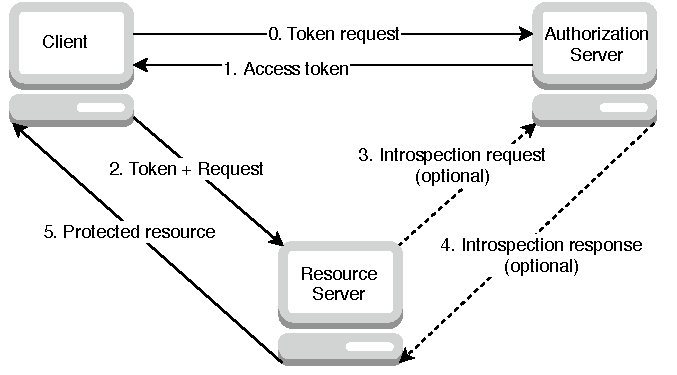
\includegraphics{images/ace.pdf}
\end{figure}

Introspection is an interesting feature of ACE since it requires less from the device
concerning verifying tokens. Instead of doing everything on its own, the device can ask
the server for additional information making the verification procedure easier. This
however requires some extra communication which is power consuming for an IoT device. To
use introspection or not is yet again an implementation issue, but authorization servers
should be both enrolled and reachable for devices to send introspection requests if
necessary.

\end{document}